\section{组合电路}
\subsection{基本逻辑门}
\begin{figure}[htbp]
	\centering
	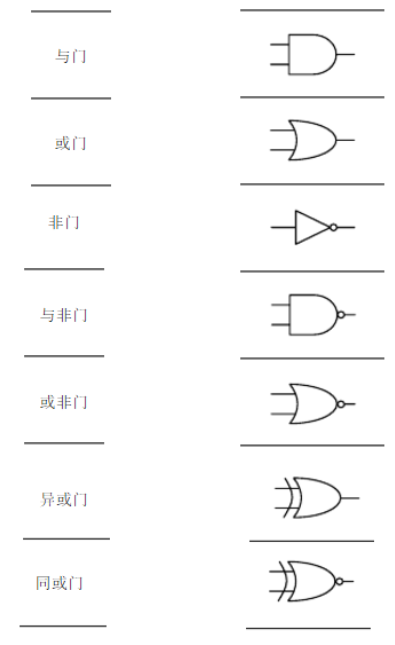
\includegraphics[width=0.6\linewidth]{fig/logic_gates.PNG}
	\caption{基本逻辑门}
\end{figure}
\subsection{布尔(Boolen)代数}
满足交换律、结合律、分配律
\[\begin{aligned}
A\ol{A}&=0 \qquad &A+\ol{A}&=1\\
A\ol{B}+\ol{A}B&=A\oplus B \qquad &AB+\ol{A}\ol{B}&=A\odot B
\end{aligned}\]
\[\begin{aligned}
A+BC&=A(1+B+C)+BC \qquad &A+\ol{A}B&=A(1+B)+\ol{A}B\\
&=(A+B)(A+C)\qquad & &=A+B
\end{aligned}\]

\subsection{卡诺(Karnaugh)图}
\begin{figure}[htbp]
	\centering
	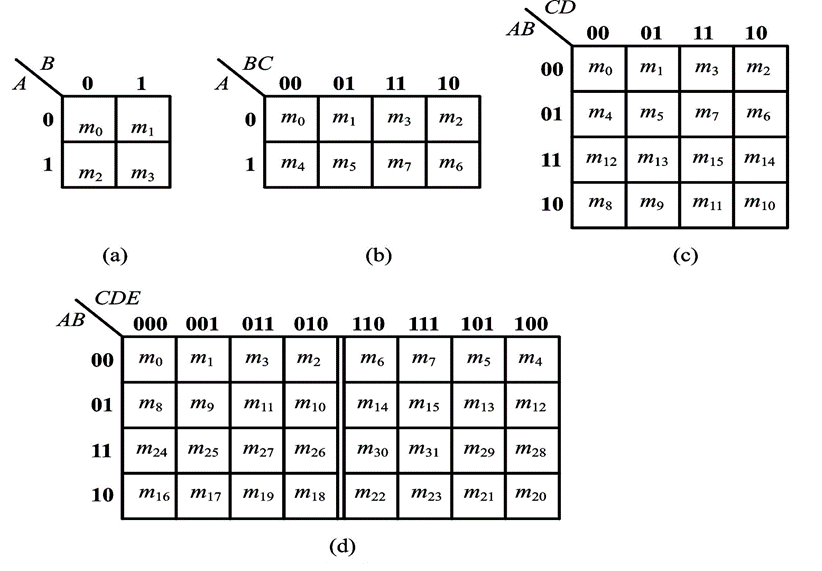
\includegraphics[width=0.8\linewidth]{fig/Karnaugh_graph.png}
	\caption{不同阶卡诺图}
\end{figure}
\begin{figure}[htbp]
	\centering
	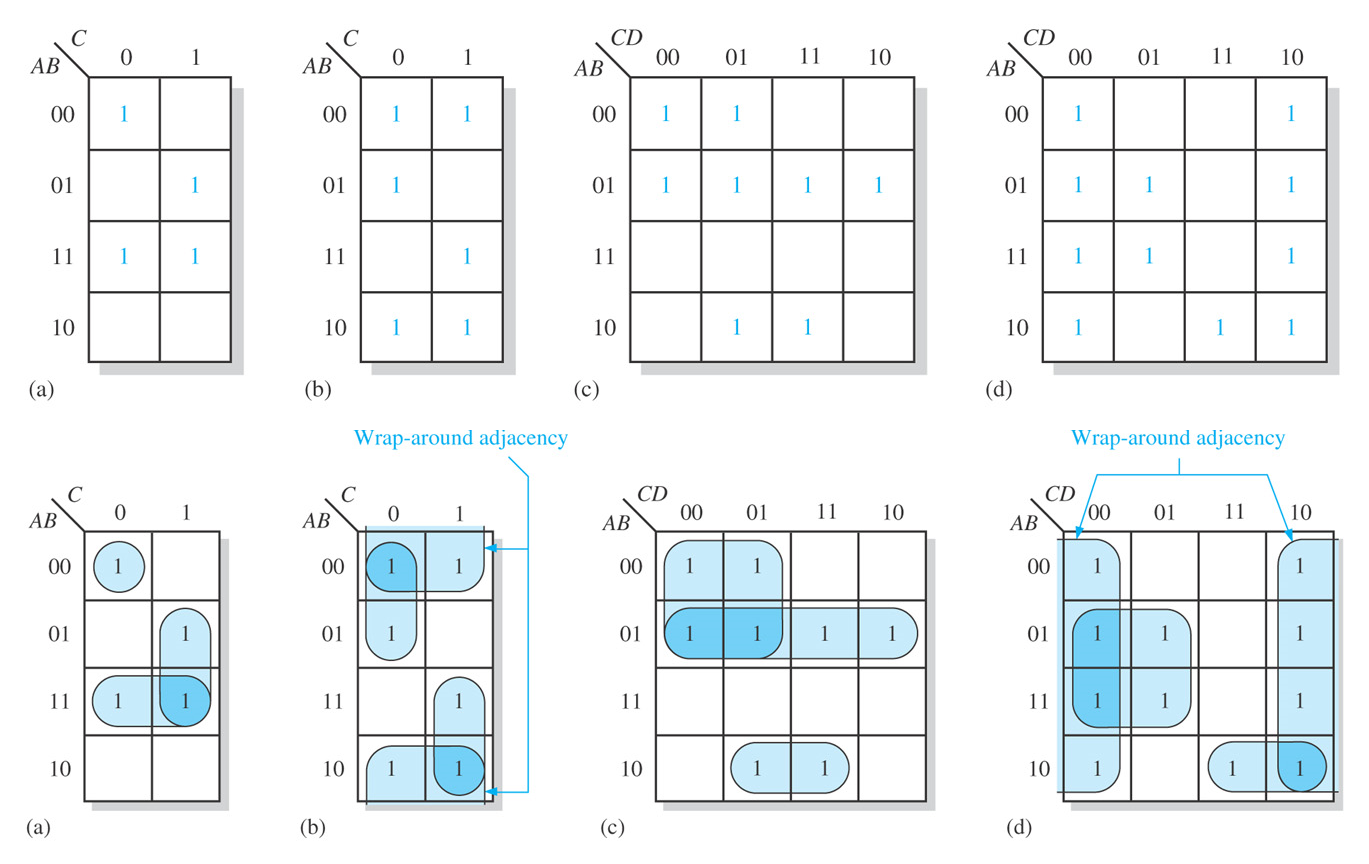
\includegraphics[width=0.8\linewidth]{fig/Karnaugh_example.png}
	\caption{Sum of Product(SOP)化简}
\end{figure}

\subsection{功能器件}
\subsubsection{加法器}
\begin{figure}[htbp]
	\centering
	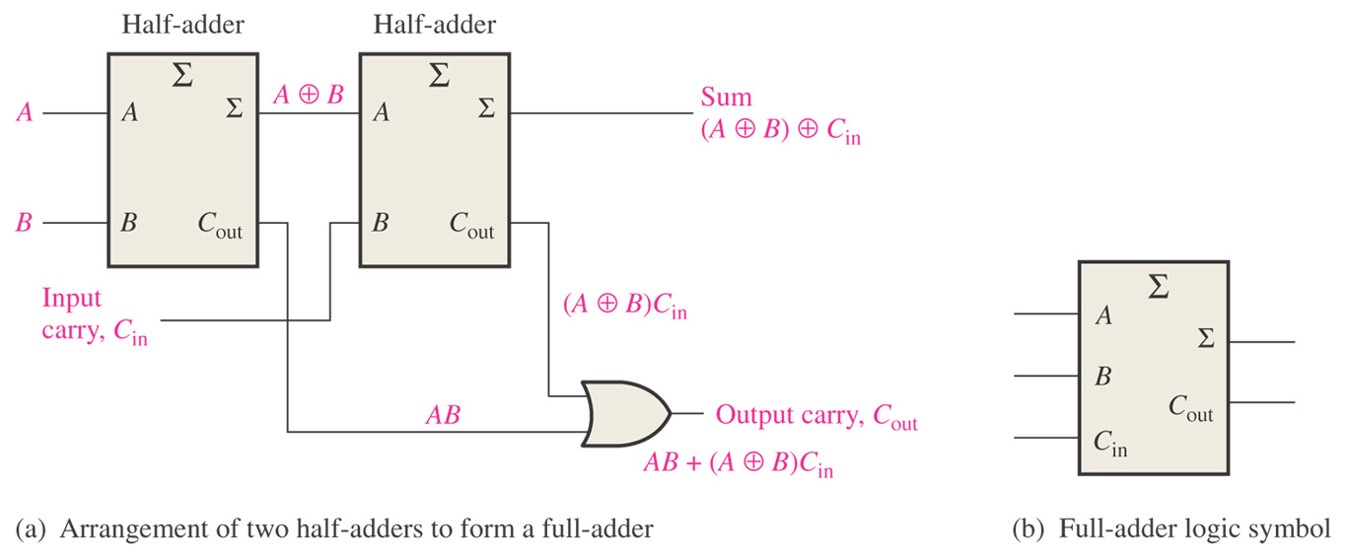
\includegraphics[width=0.8\linewidth]{fig/adder.jpg}
	\caption{半加法器与全加法器}
\end{figure}
\begin{figure}[htbp]
	\centering
	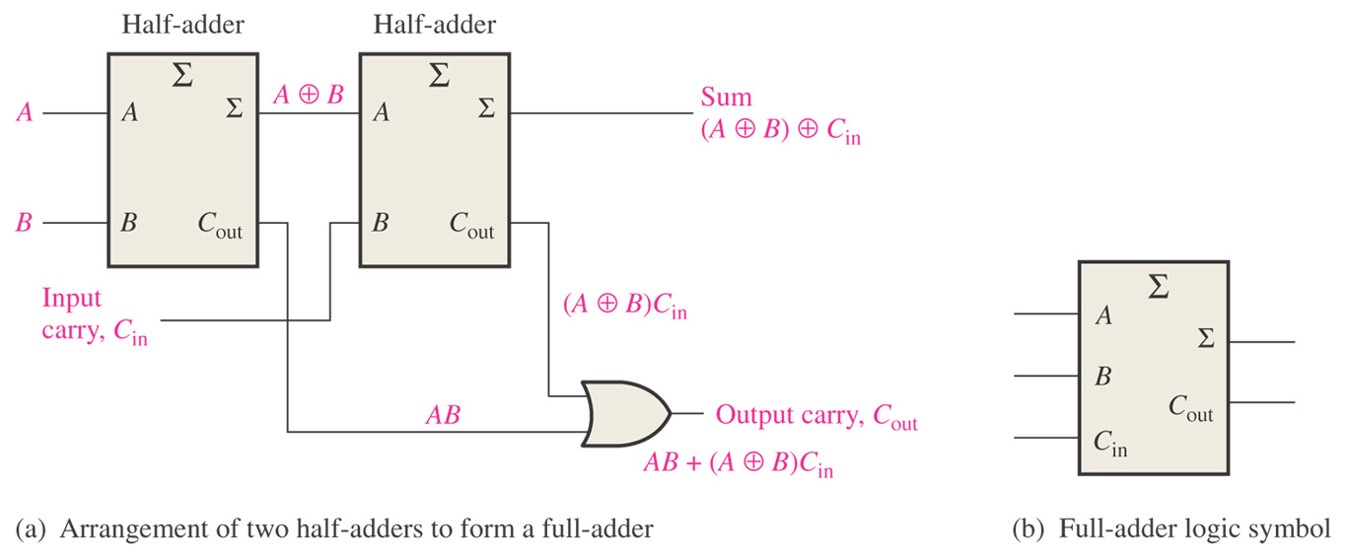
\includegraphics[width=0.8\linewidth]{fig/adder.jpg}
	\caption{异步加法器改造为同步加法器}
\end{figure}
\[\begin{aligned}
&\text{Carry generation: }&C_g&=AB\\
&\text{Carry propagation: }&C_g&=AB\\
&\text{Output carry: }&C_g&=AB\\
& &C_{in2}&=C_{out1}=C_{g1}+C_{p1}C_{in1}\\
& &C_{in3}&=C_{out2}=C_{g2}+C_{p2}C_{in2}=C_{g2}+C_{p2}(C_{g1}+C_{p1}C_{in1})
\end{aligned}\]
\subsubsection{比较器(Comparator)}
\begin{figure}[htbp]
	\centering
	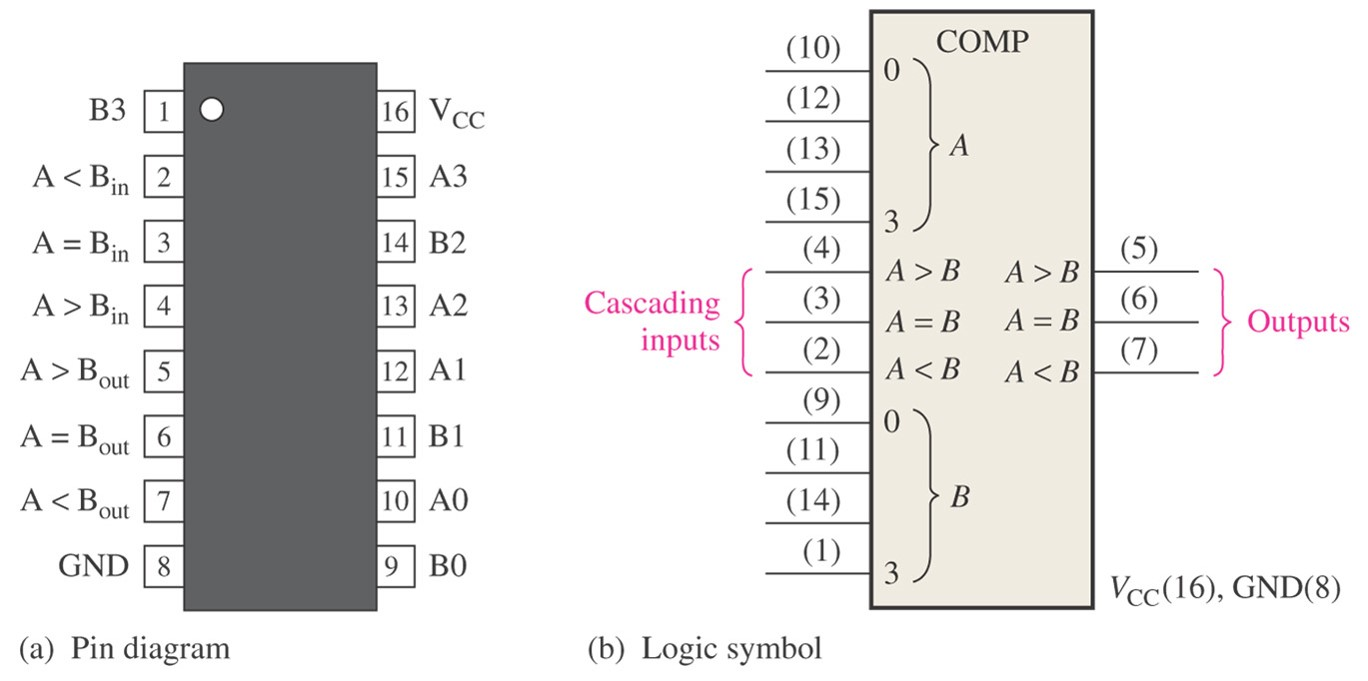
\includegraphics[width=0.8\linewidth]{fig/comparator.jpg}
	\caption{比较器}
\end{figure}
\subsubsection{译码器(Decoder)}
BCD码转对应端口输出,注意输出是反的
\begin{figure}[htbp]
	\centering
	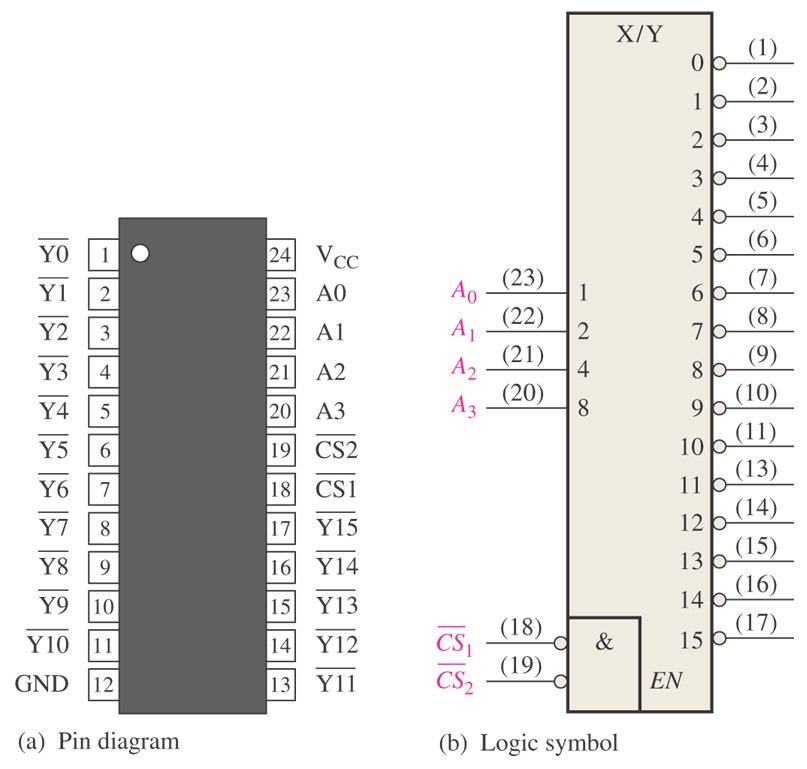
\includegraphics[width=0.5\linewidth]{fig/decoder.jpg}
	\caption{译码器}
\end{figure}
\par BCD转7段数码管
\begin{enumerate}
	\item 共阴(cathode):高电平亮
	\item 共阳(anode):低电平亮
\end{enumerate}
\subsubsection{编码器(Encoder)}
输入转BCD码
\begin{figure}[htbp]
	\centering
	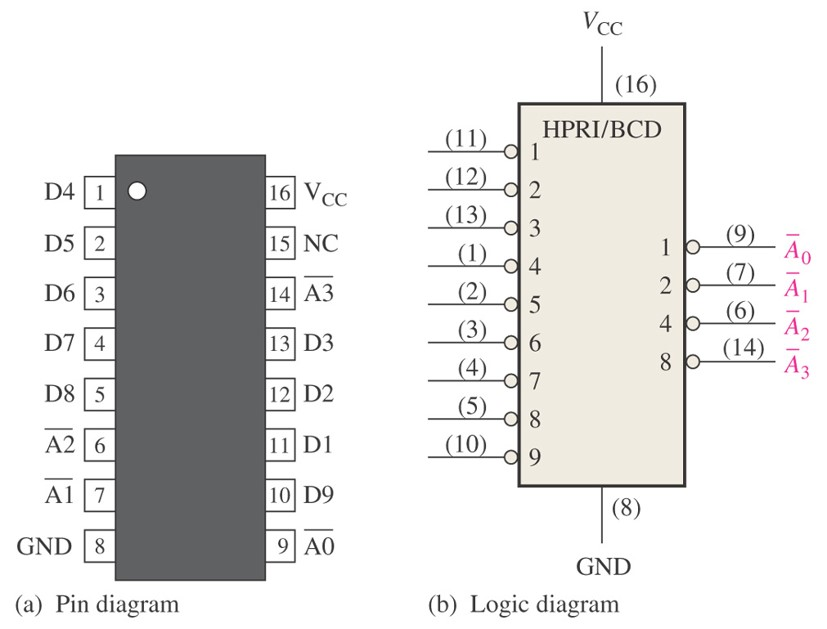
\includegraphics[width=0.6\linewidth]{fig/encoder.jpg}
	\caption{编码器}
\end{figure}
\subsubsection{选择器(Multiplexer)}
通过BCD码选择对应路输出
\begin{figure}[htbp]
	\centering
	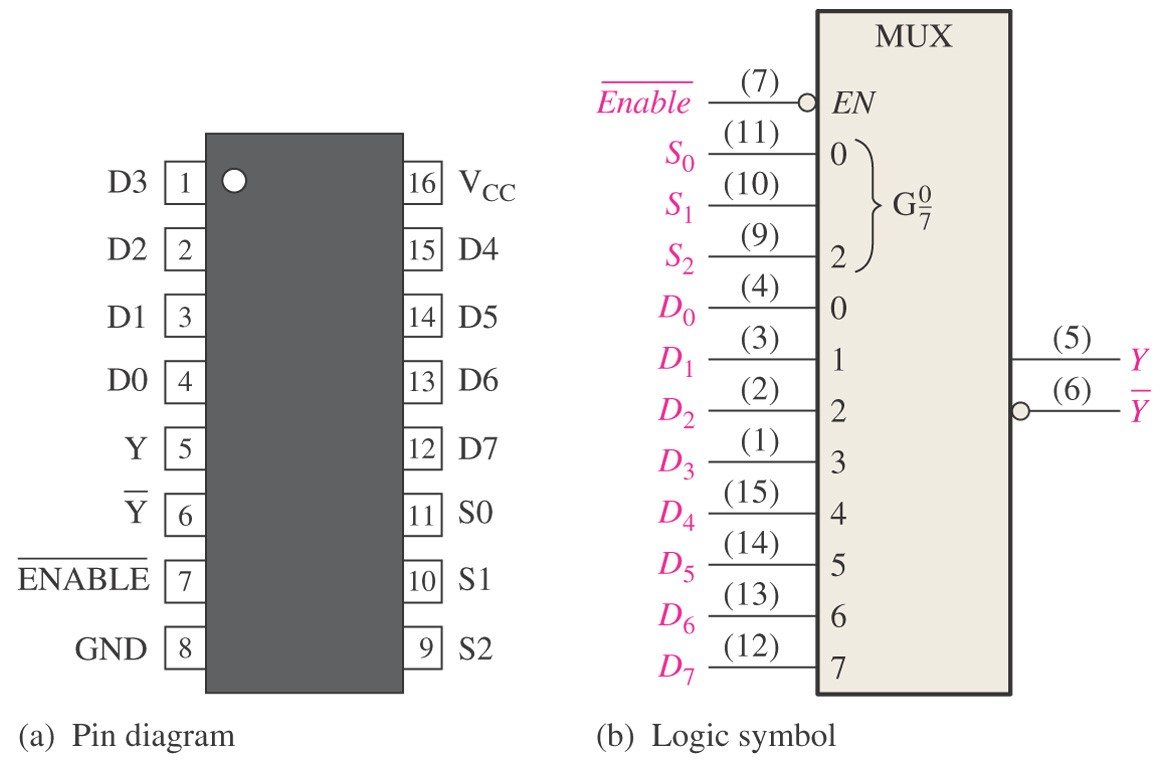
\includegraphics[width=0.6\linewidth]{fig/multiplexer.jpg}
	\caption{选择器}
\end{figure}
\subsubsection{多路分配器(Demultiplexer)}
将对应输入分配到对应输出路

\subsection{竞争与冒险}
\begin{enumerate}
	\item 竞争(race):输入到输出途径不同,延时时间不同,到达输出的时间不同
	\item 冒险(hazard):竞争结果导致逻辑电路产生错误输出
\end{enumerate}
\par 如$F=AB+\ol{A}C$,因为取非,导致两条道路时间不同,使得输出出现毛刺现象
\par 可加入冗余项以避免冒险,如改成$F=AB+\ol{A}C+BC$